% mnras_template.tex 
%
% LaTeX template for creating an MNRAS paper
%
% v3.0 released 14 May 2015
% (version numbers match those of mnras.cls)
%
% Copyright (C) Royal Astronomical Society 2015
% Authors:
% Keith T. Smith (Royal Astronomical Society)

% Change log
%
% v3.0 May 2015
%    Renamed to match the new package name
%    Version number matches mnras.cls
%    A few minor tweaks to wording
% v1.0 September 2013
%    Beta testing only - never publicly released
%    First version: a simple (ish) template for creating an MNRAS paper

%%%%%%%%%%%%%%%%%%%%%%%%%%%%%%%%%%%%%%%%%%%%%%%%%%
% Basic setup. Most papers should leave these options alone.
\documentclass[fleqn,usenatbib]{mnras}

% MNRAS is set in Times font. If you don't have this installed (most LaTeX
% installations will be fine) or prefer the old Computer Modern fonts, comment
% out the following line
\usepackage{newtxtext,newtxmath}
% Depending on your LaTeX fonts installation, you might get better results with one of these:
%\usepackage{mathptmx}
%\usepackage{txfonts}

% Use vector fonts, so it zooms properly in on-screen viewing software
% Don't change these lines unless you know what you are doing
\usepackage[T1]{fontenc}

% Allow "Thomas van Noord" and "Simon de Laguarde" and alike to be sorted by "N" and "L" etc. in the bibliography.
% Write the name in the bibliography as "\VAN{Noord}{Van}{van} Noord, Thomas"
\DeclareRobustCommand{\VAN}[3]{#2}
\let\VANthebibliography\thebibliography
\def\thebibliography{\DeclareRobustCommand{\VAN}[3]{##3}\VANthebibliography}


%%%%% AUTHORS - PLACE YOUR OWN PACKAGES HERE %%%%%

% Only include extra packages if you really need them. Common packages are:
\usepackage{graphicx}	% Including figure files
\usepackage{amsmath}	% Advanced maths commands
% \usepackage{amssymb}	% Extra maths symbols

%%%%%%%%%%%%%%%%%%%%%%%%%%%%%%%%%%%%%%%%%%%%%%%%%%

%%%%% AUTHORS - PLACE YOUR OWN COMMANDS HERE %%%%%

% Please keep new commands to a minimum, and use \newcommand not \def to avoid
% overwriting existing commands. Example:
%\newcommand{\pcm}{\,cm$^{-2}$}	% per cm-squared

%%%%%%%%%%%%%%%%%%%%%%%%%%%%%%%%%%%%%%%%%%%%%%%%%%

%%%%%%%%%%%%%%%%%%% TITLE PAGE %%%%%%%%%%%%%%%%%%%

% Title of the paper, and the short title which is used in the headers.
% Keep the title short and informative.
\title[Short title, max. 45 characters]{Identification and Classification of
Emission-line Stars in the GALAH Survey
Using Machine Learning}

% The list of authors, and the short list which is used in the headers.
% If you need two or more lines of authors, add an extra line using \newauthor
\author[P. J. Daluwathumullagamage et al.]{
Praveen Jayasuriya Daluwathumullagamage,$^{1}$\thanks{E-mail: praveen.daluwathumullagamage@students.mq.edu.au}
%A. N. Other,$^{2}$
%Third Author$^{2,3}$
%and Fourth Author$^{3}$
\\
% List of institutions
$^{1}$Macquarie University\\
%$^{2}$Department, Institution, Street Address, City Postal %Code, Country\\
%$^{3}$Another Department, Different Institution, Street %Address, City Postal Code, Country
}

% These dates will be filled out by the publisher
\date{Accepted XXX. Received YYY; in original form ZZZ}

% Enter the current year, for the copyright statements etc.
\pubyear{2015}

% Don't change these lines
\begin{document}
\label{firstpage}
\pagerange{\pageref{firstpage}--\pageref{lastpage}}
\maketitle

% Abstract of the paper
\begin{abstract}
This is a simple template for authors to write new MNRAS papers.
The abstract should briefly describe the aims, methods, and main results of the paper.
It should be a single paragraph not more than 250 words (200 words for Letters).
No references should appear in the abstract.
\end{abstract}

% Select between one and six entries from the list of approved keywords.
% Don't make up new ones.
\begin{keywords}
keyword1 -- keyword2 -- keyword3
\end{keywords}

%%%%%%%%%%%%%%%%%%%%%%%%%%%%%%%%%%%%%%%%%%%%%%%%%%

%%%%%%%%%%%%%%%%% BODY OF PAPER %%%%%%%%%%%%%%%%%%

\section{Introduction}

The GALAH survey is a large, high resolution spectroscopic survey of the Milky Way that uses the HERMES spectrograph at the Anglo Australian Telescope \citep{de2015galah}. The science goal of the survey is to unravel the formation history and evolution of the Milky Way. The most recent data release from GALAH, Data Release 3 \citep[DR3;][]{buder2021galah+}), contains more than 600,000 high-resolution spectra (R$\sim$28,000) in four passbands. 

When the number of data points (i.e., spectra) is of the order of hundreds of thousands (or millions) and when each data point has a dimensionality of several thousands (the length of a spectral data point), it becomes impractical and perhaps even unfeasible to process and analyse these data using manual methods such as naked eye observations of spectral plots. 

The GALAH survey selection function is defined by simple magnitude and Galactic latitude limits \citep{Martell+2017}, and, as a result, it is expected that a majority of spectra are typical, reflecting the underlying Galactic stellar population. Thus the identification and classification of {\em atypical} objects, such as emission-line stars, presents a serious challenge, in addition to those mentioned previously, as these spectra are outliers or anomalies in an otherwise typical set of stellar spectra.

The GALAH survey and other similar large spectroscopic surveys use data analysis pipelines to derive stellar parameters, and often use template spectra that represent typical or non-peculiar baselines. It has been demonstrated that the use of these so-called non-peculiar baselines can impact the accurate determination of effective temperature \citep{cayrel2011halpha, amarsi2018effective, giribaldi2019accurate} and stellar mass \citep{ness2016spectroscopic, bergemann2016gaia}, among other key measurements. The identification of atypical emission-line stars can thus help improve the accurate determination of these stellar parameters. To achieve this, once identified and classified, these spectra can be removed from the primary data analysis pipeline containing typical spectra, and can be reduced separately by secondary pipelines more suited for their peculiarities.

\subsection{P Cygni Stars}

P Cygni (or 34 Cygni) is a luminous blue variable star (LBV) that has been studied extensively \citep{1953PDAO....9....1B, hutchings1969expanding, elliott20225, underhill1966supergiants, mizumoto2018newly, de2001p}. The stellar spectrum of 34 Cygni is peculiar. It exhibits the characteristics of a B-type supergiant except that almost all absorption lines are blueshifted with a redshifted emission component \citep{hutchings1969expanding}. This characteristic line profile can be clearly observed in proximity to the H$\alpha$ line whose rest wavelength is at $\sim 6562.7${\rm \AA} \citep{zhang2021catalog, traven2015gaia}. 

P Cygni stars, are stars that exhibit line profiles that are similar to the characteristic profile of 34 Cygni. The spectra of these stars show characteristic absorption, emission and wide absorption sub-components \citep{zhang2021catalog}. The redshifted absorption (and blueshifted emission) counterparts to P Cygni stars have also been observed. These belong to a class of objects known as inverse P Cygni stars. These and other sub-classes of emission line stars were identified and classified by manual methods with varying levels of success \citep{1953PDAO....9....1B, van1993atlas, reipurth1996halpha, kohoutek1999catalogue, bonito2013spectroscopic}. Manual methods have since been replaced by statistical and machine learning based methods that are capable of tackling the twin problems of high volume and high dimensionality (resolution) of spectroscopic data. However significant challenges remain as it is not uncommon that manual methods are still being used for the identification and classification of emission-line stars even in modern data-sets with thousands of stars, with \citet{zhang2021catalog} being a recent example.

\subsection{A Brief Review of Machine Learning Based Methods}

The twin problems of high data volume and high data dimensionality (due to high resolution), as well as the detection of atypical signals or data points in significantly larger, more typical populations of data presents itself well to modern machine-learning methods, particularly to anomaly detection, as well as to clustering methods (unsupervised learning). 

However recent attempts such as the use of k-means clustering on high-resolution APOGEE infrared spectroscopic data (R$\sim$22,500) \citep{garcia2018machine}, taken as part of the Sloan Digital Sky Survey (SDSS) \citep{eisenstein2001spectroscopic, blanton2017sloan} demonstrate that while k-means was successful in clustering dwarfs, sub-giants, red clump and red giant branch stars into distinct classes without requiring labeled training data, the method was unable to cluster emission-line stars. One major limitation of this approach is that a discrete classification in flux space does not result in a neat organisation in parameter space, which implies that the authors were not able to link spectral features such as spectroscopic morphologies to the machine learning parameter space. 

The LAMOST survey is a low-resolution spectroscopic survey with 10 million Milky Way stars as potential survey spectra. \citet{zhang2021catalog} were able to use a training and test set (labelled spectra) comprising of 5915 samples for spectral classification. This training set was based on data released by \citet{hou2016catalog}, who developed the data set by using a combination of empirical rules and visual examination of 10,000 LAMOST spectra. The labelled data, including seven P Cygni and inverse P Cygni spectra identified by \citeauthor{hou2016catalog} was used by \citeauthor{zhang2021catalog} for supervised machine learning algorithms. Ten different supervised learning methods were then applied to this data set including including KNN (K-Nearest Neighbor), RF (Random Forest), AdaBoost, Naive Bayes (MultinomialNB, GaussianNB, BernoulliNB), logistic regression, SVM (Support Vector Machine) and Artificial Neural Network (Single-hidden Layer, Three-hidden Layer).

\citeauthor{zhang2021catalog}, however, note that the k-nearest neighbour and random forest methods outperformed all other methods. These two supervised machine learning models were then applied to 498,588 spectra, resulting in 56,574 potential H$\alpha$ emission-line spectra. These spectra were then visually inspected, with a final candidate list of 30,048 H$\alpha$ emission-line spectra. Despite the use of a number of machine learning methods, the authors fell back on manual visual inspection of spectra in building the training set, and during the classification of the identified potential H$\alpha$ emission-line spectra. 



\section{Methods, Observations, Simulations etc.}

Normally the next section describes the techniques the authors used.
It is frequently split into subsections, such as Section~\ref{sec:maths} below.

\subsection{Maths}
\label{sec:maths} % used for referring to this section from elsewhere

Simple mathematics can be inserted into the flow of the text e.g. $2\times3=6$
or $v=220$\,km\,s$^{-1}$, but more complicated expressions should be entered
as a numbered equation:

\begin{equation}
    x=\frac{-b\pm\sqrt{b^2-4ac}}{2a}.
	\label{eq:quadratic}
\end{equation}

Refer back to them as e.g. equation~(\ref{eq:quadratic}).

\subsection{Figures and tables}

Figures and tables should be placed at logical positions in the text. Don't
worry about the exact layout, which will be handled by the publishers.

Figures are referred to as e.g. Fig.~\ref{fig:example_figure}, and tables as
e.g. Table~\ref{tab:example_table}.

% Example figure
\begin{figure}
	% To include a figure from a file named example.*
	% Allowable file formats are eps or ps if compiling using latex
	% or pdf, png, jpg if compiling using pdflatex
	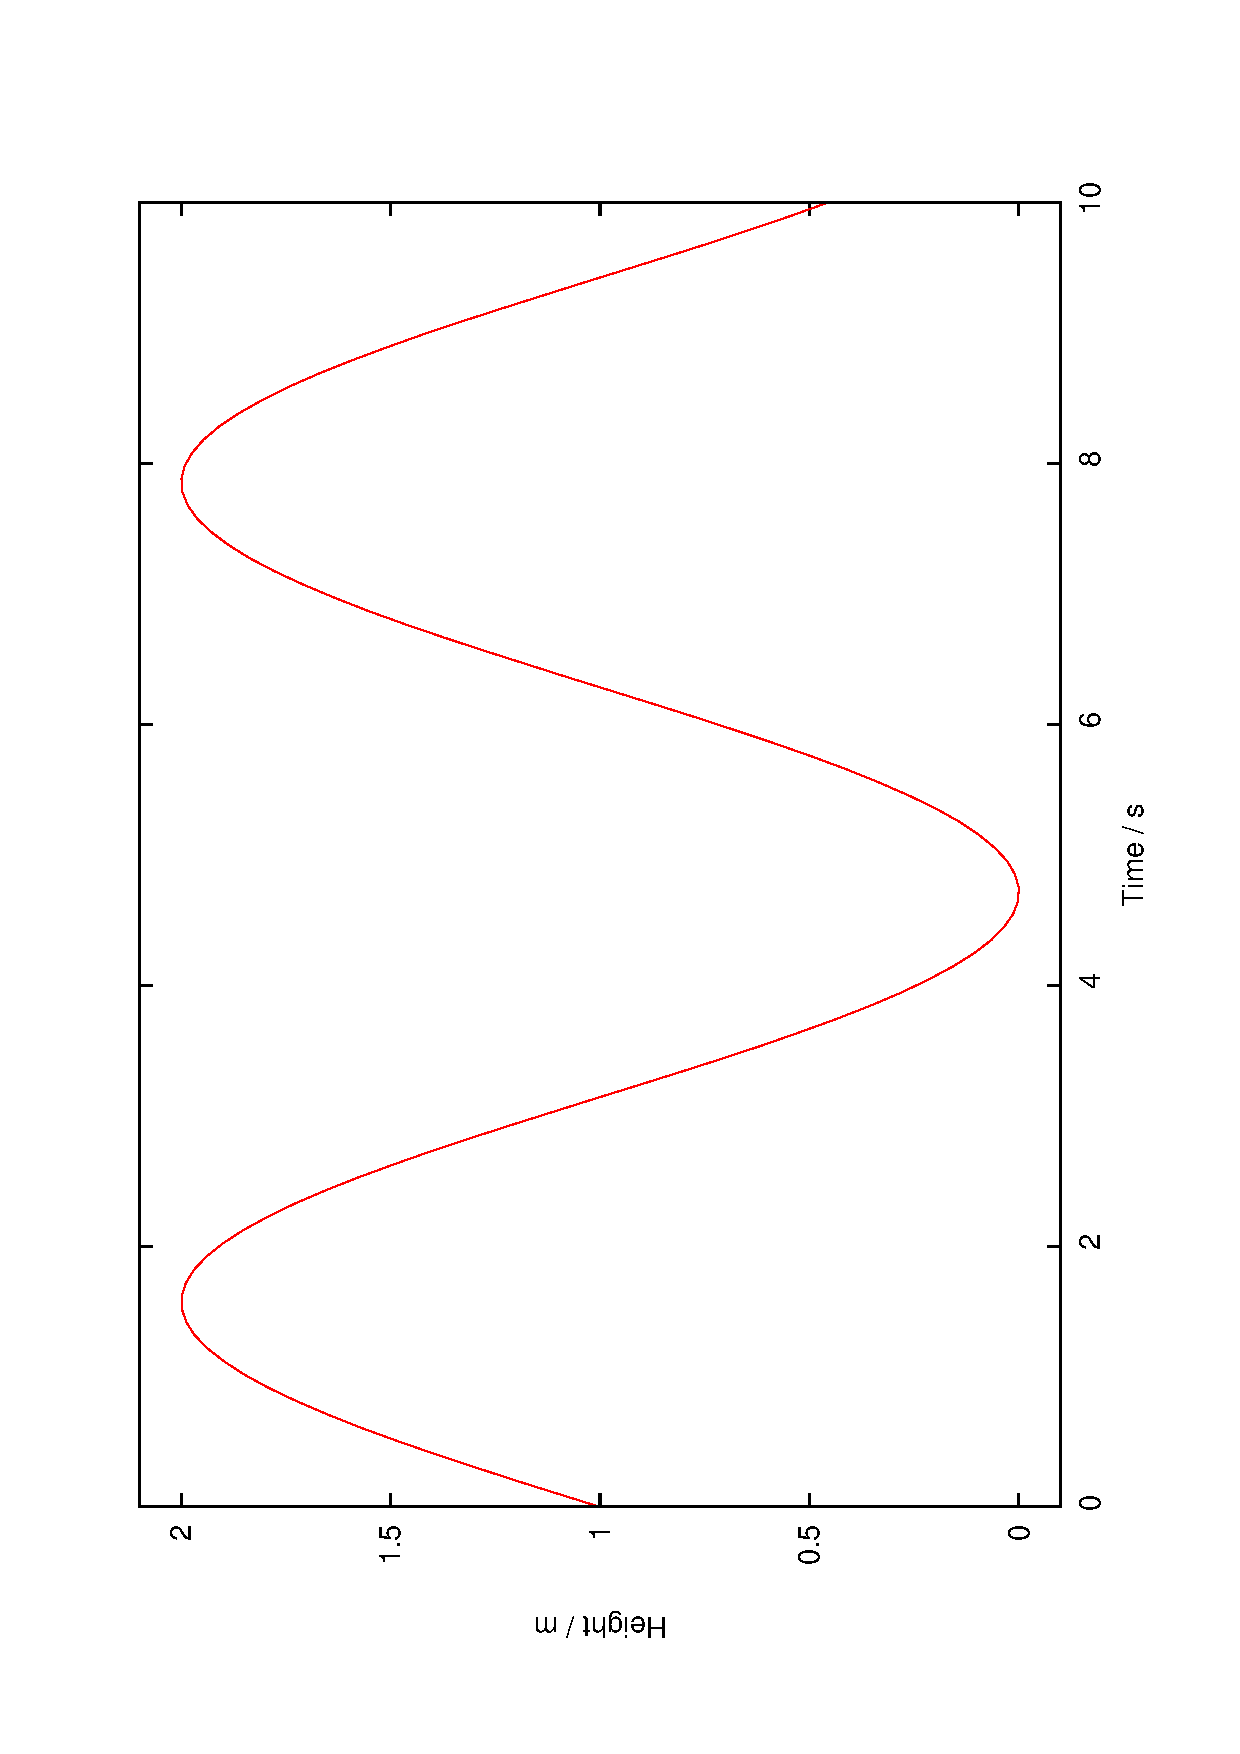
\includegraphics[width=\columnwidth]{example}
    \caption{This is an example figure. Captions appear below each figure.
	Give enough detail for the reader to understand what they're looking at,
	but leave detailed discussion to the main body of the text.}
    \label{fig:example_figure}
\end{figure}

% Example table
\begin{table}
	\centering
	\caption{This is an example table. Captions appear above each table.
	Remember to define the quantities, symbols and units used.}
	\label{tab:example_table}
	\begin{tabular}{lccr} % four columns, alignment for each
		\hline
		A & B & C & D\\
		\hline
		1 & 2 & 3 & 4\\
		2 & 4 & 6 & 8\\
		3 & 5 & 7 & 9\\
		\hline
	\end{tabular}
\end{table}


\section{Conclusions}

The last numbered section should briefly summarise what has been done, and describe
the final conclusions which the authors draw from their work.

\section*{Acknowledgements}

The Acknowledgements section is not numbered. Here you can thank helpful
colleagues, acknowledge funding agencies, telescopes and facilities used etc.
Try to keep it short.

%%%%%%%%%%%%%%%%%%%%%%%%%%%%%%%%%%%%%%%%%%%%%%%%%%
\section*{Data Availability}

 
The inclusion of a Data Availability Statement is a requirement for articles published in MNRAS. Data Availability Statements provide a standardised format for readers to understand the availability of data underlying the research results described in the article. The statement may refer to original data generated in the course of the study or to third-party data analysed in the article. The statement should describe and provide means of access, where possible, by linking to the data or providing the required accession numbers for the relevant databases or DOIs.




%%%%%%%%%%%%%%%%%%%% REFERENCES %%%%%%%%%%%%%%%%%%

% The best way to enter references is to use BibTeX:

\bibliographystyle{mnras}
\bibliography{example} % if your bibtex file is called example.bib


% Alternatively you could enter them by hand, like this:
% This method is tedious and prone to error if you have lots of references
%\begin{thebibliography}{99}
%\bibitem[\protect\citeauthoryear{Author}{2012}]{Author2012}
%Author A.~N., 2013, Journal of Improbable Astronomy, 1, 1
%\bibitem[\protect\citeauthoryear{Others}{2013}]{Others2013}
%Others S., 2012, Journal of Interesting Stuff, 17, 198
%\end{thebibliography}

%%%%%%%%%%%%%%%%%%%%%%%%%%%%%%%%%%%%%%%%%%%%%%%%%%

%%%%%%%%%%%%%%%%% APPENDICES %%%%%%%%%%%%%%%%%%%%%

\appendix

\section{Some extra material}

If you want to present additional material which would interrupt the flow of the main paper,
it can be placed in an Appendix which appears after the list of references.

%%%%%%%%%%%%%%%%%%%%%%%%%%%%%%%%%%%%%%%%%%%%%%%%%%


% Don't change these lines
\bsp	% typesetting comment
\label{lastpage}
\end{document}

% End of mnras_template.tex
